\documentclass[aspectratio=169, 8pt,t]{beamer}
\graphicspath{{figures/}} % Setting the graphicspath

% Theme settings
\usetheme{Madrid}
\usecolortheme{default}
\setbeamertemplate{navigation symbols}{}   % removes navigation symbols such as 'next page'
\setbeamertemplate{footline}{}             % remove line with name, date, page nr.
\setbeamercolor*{frametitle}{bg=white}     % remove background from frametitle
\usepackage{caption}
% \captionsetup[figure]{labelformat=empty}% redefines the caption setup of the figures environment in the beamer class.
\setbeamersize{text margin left=20pt,text margin right=10pt}
\usefonttheme[onlymath]{serif} % makes beamer math look like article math
\usepackage{hyperref}


%======================= title page info =======================
\title{An NNPDF4.0 determination of $\alpha_s$ -- methodologies \& status}
\date{NNPDF collaboration meeting  \\[0.1cm] Amsterdam, 24 February 2024}
\author{Roy Stegeman}
\institute{\small The University of Edinburgh}


%======================= page numbering =======================
\addtobeamertemplate{navigation symbols}{}{ \usebeamerfont{footline}
  \insertframenumber / \inserttotalframenumber \hspace*{2mm} \\ \vspace*{1mm}
}


%=================================== colors ====================================
\definecolor{RoyBlue}{RGB}{22, 46, 69}
\definecolor{RoyGrey}{RGB}{64, 88, 128}

\newcommand{\hlme}[1]{{\color{red}\bf #1}} % highlight me

\setbeamercolor{structure}{fg=RoyBlue} % itemize, enumerate, etc
\setbeamercolor{frametitle}{fg=RoyGrey}
\setbeamercolor{section in head/foot}{bg=RoyBlue}


%======================= add progress dots to headline =========================
\setbeamertemplate{headline}{%
    \begin{beamercolorbox}[ht=4mm,dp=4mm]{section in head/foot}
        \insertnavigation{\paperwidth}
    \end{beamercolorbox}%
}%
\makeatother


%======================= add section title page ================================
\AtBeginSection[]{
  \begin{frame}
  \vfill
  \centering
    \usebeamerfont{title}\insertsection\par%
  \vfill
  \end{frame}
}


%=================================== titlepage =================================
\titlegraphic{\vspace*{6mm}
  
\includegraphics[height=1.5cm]{logos/edi_logo.png} \hspace{10mm}
  % 
\includegraphics[height=0.8cm]{logos/nnpdf_logo_official.pdf} \hspace{10mm}
  
\includegraphics[height=1.5cm]{logos/higgs_logo.jpg}
}

\defbeamertemplate{title page}{noinstitute}[1][]
{
  \vbox{}
  \vfill
  \begingroup
    \centering
    \begin{beamercolorbox}[sep=8pt,center,#1]{title}
      \usebeamerfont{title}\inserttitle\par%
      \ifx\insertsubtitle\@empty%
      \else%
        \vskip0.25em%
        {\usebeamerfont{subtitle}\usebeamercolor[fg]{subtitle}\insertsubtitle\par}%
      \fi%
    \end{beamercolorbox}%
    \vskip2em\par
    \begin{beamercolorbox}[sep=0pt,center,#1]{author}
      \usebeamerfont{author}\insertauthor
    \end{beamercolorbox}
  \begin{beamercolorbox}[sep=0pt,center,#1]{author}
    \usebeamerfont{institute}\insertinstitute
  \end{beamercolorbox}
  \vspace*{8pt}
  \vspace*{16pt}
    \begin{beamercolorbox}[sep=0pt,center,#1]{date}
      \usebeamerfont{date}\insertdate
    \end{beamercolorbox}\vskip0.5em
    {\usebeamercolor[fg]{titlegraphic}\inserttitlegraphic\par}
  \endgroup
  \vfill
}

\makeatletter
\setbeamertemplate{title page}[noinstitute][colsep=-4bp,rounded=true,shadow=\beamer@themerounded@shadow]
\makeatother


\begin{document}
{
\setbeamertemplate{headline}{} % remove headline from titlepage
\begin{frame}
  \titlepage
\end{frame}
}

\setbeamertemplate{enumerate items}[default]

\pgfdeclarelayer{bg}    % declare background layer
\pgfsetlayers{bg,main}  % set the order of the layers (main is the standard layer)


% SLIDES =======================================================================


\begin{frame}{Three different methodologies}
  \begin{itemize}
    \item Correlated replica method \href{https://arxiv.org/abs/1802.03398}{\textcolor{gray}{[NNPDF Collaboration (2018); 1802.03398]}}
    \item Theory covariance method \href{https://arxiv.org/abs/2105.05114}{\textcolor{gray}{[Ball \& Pearson (2021); 2105.05114]}}
    \item SIMUnet (no results in these slides) \href{https://arxiv.org/abs/2201.07240}{\textcolor{gray}{[Iranipour \& Ubiali (2022); 2201.07240]}}
  \end{itemize}
\end{frame}


\begin{frame}{Correlated replica method}
  Determining $\alpha_s$ with a fixed input PDF results in underestimated uncertainty
  \begin{figure}
    \centering
    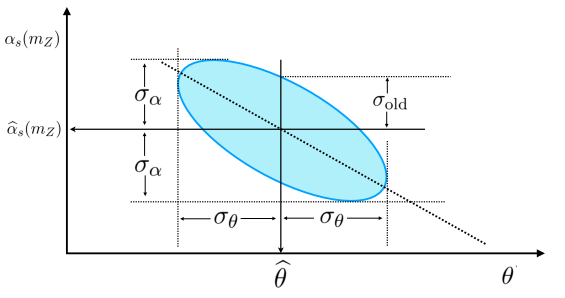
\includegraphics[width=0.7\textwidth]{figures/alphaspdfcorplot.png}
  \end{figure}
\end{frame}


\begin{frame}{Correlated replica method}
  \begin{columns}
    \column{0.5\textwidth}
    1. Produce fits to a data replica, $D^k$ at different values of $\alpha_s$, such that we can determine $\alpha_s^{(k)}=\operatorname{argmin}\left[\chi^{2(k)}\left(\alpha_s\right)\right]$ \\\vspace*{1em}
    2. Perform quadratic fit to $\chi^2$ profiles \\
    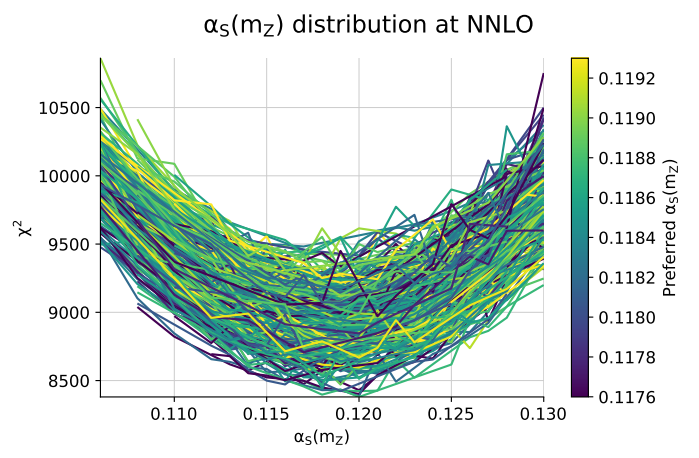
\includegraphics[width=0.9\textwidth]{figures/parabolaplotnnpdf31.png}
    \column{0.5\textwidth}
    3. Analyze the resulting probability distribution \\
    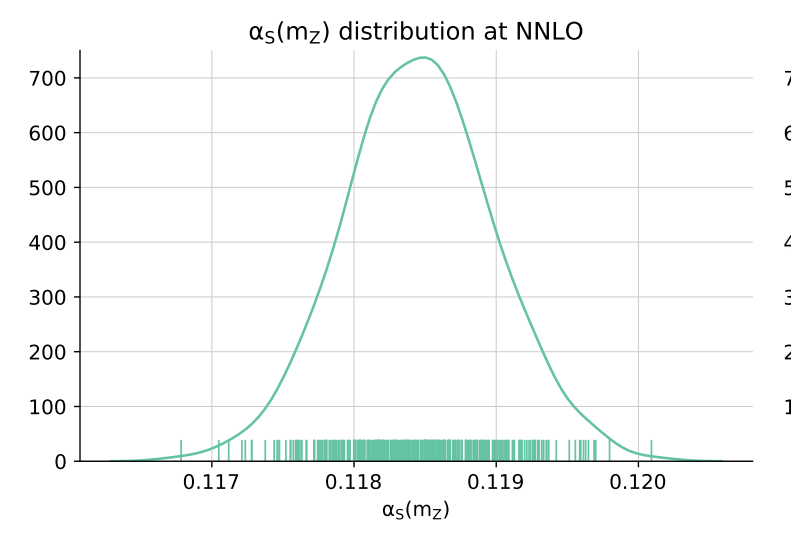
\includegraphics[width=0.9\textwidth]{figures/alphasnnpdf31result.png}
  \end{columns}

  % batch minimization

\end{frame}


\begin{frame}{Correlated replica method}
  % NNPDF3.1: 0.1185 ± 0.0005


  % results table here

  % 68% c.i MHOU   : 0.12101 to 0.12447 (large non-Gaussianity)
  % 68% c.i no MHOU: 0.12085 to 0.12247



\end{frame}

\begin{frame}{Way forward?}
  Problems:
  \begin{itemize}
    \item Disagreement between datasets (still to confirm with new pipeline+mhou)
    \item Disagreement between methodologies
    \item CRM: Best alphas central data vs best alphas validation replicas
    \item CRM: Fixed t0 (not done in 3.1 determination) and MHOU covmat across all values of
    \item SIMUnet: How to do stopping?
  \end{itemize}

  Things to do:
  \begin{itemize}
    \item TCM: Go beyond quadratic expansion in nuisance parameter
    \item Repeat for more datasets (to test if MHOU solves disagreement)
    \item Produce more theories: N3LO, MHOU at alphas other than 0.118, more alphas values
    \item \ldots?
  \end{itemize}

  Let's discuss\ldots
\end{frame}




\end{document}
